
%(BEGIN_QUESTION)
% Copyright 2007, Tony R. Kuphaldt, released under the Creative Commons Attribution License (v 1.0)
% This means you may do almost anything with this work of mine, so long as you give me proper credit

An instrument called a {\it Time-Domain Reflectometer}, or {\it TDR}, may be used to measure the length of an unterminated cable by generating a very brief voltage pulse and waiting to receive the reflected pulse ``bounced'' back from the cable's end.  The duration of this pulse is so brief that it is done and over before the signal has a chance to travel down the cable and back:

$$\includegraphics[width=15.5cm]{i02181x01.eps}$$

Build a computer spreadsheet to calculate cable length, given the echo time (entered in microseconds) measured by a TDR, and the velocity factor of the cable.  An example spreadsheet layout is shown here (the cell fill coloring is just for looks, distinguishing the {\it calculated} value of cable length from the {\it entered} values of echo time and velocity factor):

$$\includegraphics[width=15.5cm]{i02181x02.eps}$$

\vskip 20pt \vbox{\hrule \hbox{\strut \vrule{} {\bf Suggestions for Socratic discussion} \vrule} \hrule}

\begin{itemize}
\item{} How could you {\it test} your spreadsheet cable-length calculator for accuracy (to verify you haven't made any mistakes) once you've entered all your equations?
\item{} Note that there is no entry on this spreadsheet for the {\it frequency} of the TDR's test signal, or the width of that signal's pulse duration.  Explain why these parameters are not a part of the cable length calculation.
\item{} What would a {\it real} oscilloscope screenshot look like in this scenario, with a real cable?
\end{itemize}

\underbar{file i02181}
%(END_QUESTION)





%(BEGIN_ANSWER)

\begin{itemize}
\item{} {\bf Cell R1C1:} {\tt Echo time =}
\item{} {\bf Cell R1C3:} {\tt (microseconds)}
\item{} {\bf Cell R2C1:} {\tt Velocity factor =}
\item{} {\bf Cell R2C3:} {\tt (unitless)}
\item{} {\bf Cell R4C1:} {\tt Cable length =}
\item{} {\bf Cell R4C2:} {\tt = 983.571056 * R1C2 * R2C2 / 2}
\item{} {\bf Cell R4C3:} {\tt (feet)}
\end{itemize}

%(END_ANSWER)





%(BEGIN_NOTES)

Distance, velocity, and time are related by the following formula:

$$x = vt$$

Knowing that we are intereted in the round-trip signal reflection time, we must cut the measured time in half, because the measured time represents round-trip cable length (down and back up):

$$x = {vt \over 2}$$

Given time in microseconds and solving for $x$ in feet means we must use the velocity of light in British units (983,571,056 ft/sec):

$$x = {983571056 t \over 2}$$

Including velocity factor $k$ to account for the slower velocity of propagation:

$$x = {983571056 kt \over 2}$$

Since we are told to make the spreadsheet input time in microseconds rather than seconds, we must include the ``micro'' power of ten ($1 \times 10^{-6}$) as a factor in this equation:

$$x = {(983571056)(1 \times 10^{-6}) kt \over 2}$$

$$x = {983.571056 kt \over 2}$$

%INDEX% Computer spreadsheet exercise: transmission line length calculator
%INDEX% Electronics review: characteristic impedance of transmission line
%INDEX% Electronics review: surge impedance of transmission line

%(END_NOTES)


